\documentclass[a4paper]{article} 
\addtolength{\hoffset}{-2.25cm}
\addtolength{\textwidth}{4.5cm}
\addtolength{\voffset}{-3.25cm}
\addtolength{\textheight}{5cm}
\setlength{\parskip}{0pt}
\setlength{\parindent}{0in}

\usepackage{blindtext} % Package to generate dummy text
\usepackage{charter} % Use the Charter font
\usepackage[utf8]{inputenc} % Use UTF-8 encoding
\usepackage{microtype} % Slightly tweak font spacing for aesthetics
\usepackage[english]{babel} % Language hyphenation and typographical rules
\usepackage{amsthm, amsmath, amssymb} % Mathematical typesetting
\usepackage{float} % Improved interface for floating objects
\usepackage{subcaption}
\usepackage[final, colorlinks = true, 
linkcolor = black, 
citecolor = black]{hyperref} % For hyperlinks in the PDF
\usepackage{graphicx, multicol} % Enhanced support for graphics
\usepackage{xcolor} % Driver-independent color extensions
\usepackage{marvosym, wasysym} % More symbols
\usepackage{rotating} % Rotation tools
\usepackage{censor} % Facilities for controlling restricted text
\newcommand{\note}[1]{\marginpar{\scriptsize \textcolor{red}{#1}}} % Enables comments in red on margin
\newcommand{\F}[0]{$\mathcal{F}$ }
\newcommand{\G}[0]{$\mathcal{G}$ }
\newcommand{\C}[0]{$\mathcal{C}$ }
\definecolor{colkeyword}{rgb}{0,0.4,0}
\definecolor{colname}{rgb}{0.4,0.4,0}
\definecolor{coltype}{rgb}{0.4,0,0.4}
\definecolor{coloperators}{rgb}{0,0,1.0}
\definecolor{colscopes}{rgb}{0.4,0,0}

% Title Page
\title{Documentation Lean Hammer}
\author{Phillip Lippe}


\begin{document}
\maketitle
\tableofcontents
\newpage

\section*{General remarks}
This documentation contains a description of a hammer designed for the Dependent Type Theory of Lean. The aim is to use fast theorem provers of lower-level logics (like FOL, TH0 etc.) to support the user of finding proofs in Lean. \\

The current code can be found on this github repository \href{https://github.com/phlippe/Lean_hammer}{https://github.com/phlippe/Lean\_hammer}. It is recommended to take a look at the code while reading this documentation. The code is commented for giving low-level details, but the high-level overview can be found in this documentation.\\

\subsection*{Overview}

In general, there are two development branches for the Lean hammer. When this project started, we focused on a similar approach to which is already implemented in the Coq proof assistant \cite{CoqHammer}. In there, we have a pipeline designed for translating Dependent Type Theory to First-order logic with equality. This approach is described in Section~\ref{sec:specific_pipeline_DTT_FOL}.\\
The second approach, which was introduced later and is still in construction, is designing a pipeline which allows a step-wise translation to FOL where we can stop at any time. Thereby, we would first translate DTT to e.g. the high-order logic TH1. This can be translated to e.g. TH0 or TF1, and finally we end up in TF0 or plain FOL. This would allow us to use a much greater variety of theorem provers, and maybe makes the translation process more tractable. The current state of this idea is presented in Section~\ref{sec:general_pipeline}. 

\subsection*{Contact}
If you have any questions about the code/design/etc., do not hesitate to contact me by \href{mailto:phillip.lippe@googlemail.com}{phillip.lippe@googlemail.com}.

\newpage
\section{Specific pipeline DTT to FOL}
\label{sec:specific_pipeline_DTT_FOL}
\subsection{Approach}
The first version of the Lean hammer implements a direct translation from DTT to FOL. The approach follows the \href{https://link.springer.com/article/10.1007/s10817-018-9458-4}{Coq hammer paper} \cite{CoqHammer} by introducing an intermediate representation. Details are explained along the code description.
% \subsection{Implementation}
\subsection{Code structure}
The code is split into multiple files
\begin{itemize}
	\item \texttt{leanhammer.lean}: Main file combining all functions for testing. In here, we include examples of translation, and show the usage of the overall system.
	\item \texttt{problem\_translation.lean}: Summarizes the steps for translating a problem into FOF. Note that this file should mostly be independent of the actual encoding of the first-order logic.
	\item \texttt{premise\_selection.lean}: Implementation of strategies for selecting the most relevant premises/axioms. Still in a very early form. Might be moved into C/C++ code for performance gain. 
	\item \texttt{import\_export.lean}: Handling functions for the import and export of files (communication to first-order provers)
\end{itemize}

Next to the general files, there are several functions that directly interact with the underlying FOF encoding. Currently, only the TPTP3 encoding is fully supported that can be processed by theorem provers like E. The implementation for that is structured as follows:
\begin{itemize}
	\item \texttt{tptp.lean}: Summarizes data structures for simple first-order formula and their representation in the TPTP format
	\item \texttt{translation\_tptp.lean}: Functions for translating expressions into FOF. This include the hammer functions \F, \C and \G of  \cite{CoqHammer} (described in detail below). 
	\item \texttt{simplification\_tptp.lean}: Simplification/optimization of terms for TPTP encoded first-order formula. Here for example terms that only occur together (like \texttt{has\_add(nat)}), are replaced with a new constant name.
\end{itemize}

All the mentioned steps in the previous descriptions will be explained below.

\subsection{Low-level translation}

In this section, the translation of single units (here Lean expressions) is described. This part is highly inspired by \cite{CoqHammer}.

\subsubsection{Translating expressions into intermediate representations}
\label{sec:term_translation}
The Coq paper relies on an intermediate representation called $\text{CIC}_0$ in which the DTT expressions are encoded with the help of the functions \F, \C and \G. In this implementation of the Lean hammer, a similar approach is used. The data structures of the intermediate representations, which are closely related to FOL, can be found in \texttt{tptp.lean}. An axiom for example consists of a name and a formula in FOL, which again can consist of multiple formula or terms. The set of all axioms and constants which were introduced in the translation process, are summarized in the data structure \texttt{hammer\_state}. To this structure, axioms are successively added during the translation.\\
For the export of this data structure to other theorem provers, the function \texttt{to\_format} is defined for the structures \texttt{folform} and \texttt{folterm} which returns the corresponding TPTP FOL representation of the formula/terms as a string. This can be used to export the translated axioms and use them as input to e.g. E \cite{EProver}.\\

The main translation happens in the functions \texttt{hammer\_c}, \texttt{hammer\_g} and \texttt{hammer\_f} which implement \C, \G and \F of \cite{CoqHammer}. In general, the functions have the following purpose:
\begin{itemize}
	\item \F encodes propositions as FOL formulas. Therefore, it takes a Lean expression which has to be of type \texttt{Prop} (e.g. \texttt{1+1=2}), and translates it into the previously defined data structures. Note that for expressions that are not propositions, we can only include them as type guard with \G. For more details how declarations/other expressions in Lean are used, see Section~\ref{sec:axiom_expressions}.
	\item \C takes a Lean expression, and translates it into a FOL term. The function \F makes use of it while translating (e.g. for translating \texttt{1+1=2}, it calls \C on the expression \texttt{1+1} and \texttt{2}).
	\item \G encodes type guards on FOL terms. This includes for example that \texttt{1} is of type $\mathbb{N}$. The corresponding proposition used for this is noted by $T$ here, and we add new axioms as for example $t(1,\mathbb{N})$. When translating declarations, these guards are used to limits the possible input arguments to which the declaration/function holds. For an example, see Appendix~\ref{sec:fol_examples} formula \texttt{\_fresh.265.4450}. Note that these type constraints get redundant if we use language that include types, as e.g. TF0. 
\end{itemize}

The implementation of these functions are closely related to the definitions in \cite{CoqHammer}. For details, we refer to the code.

\subsubsection{Term optimizations}

The translation process described in the previous section might be inefficient in some cases. Take for example the number \texttt{2}. From Lean, the expression is translated to:

\begin{verbatim}
	a(a(a('bit0','nat'),'nat.has_add'),a(a('has_one.one','nat'),'nat.has_one'))
\end{verbatim}

This term already contains 5 applications, and is most times not necessary.  Therefore, we apply the following simplification rule:

\begingroup
\leftskip4em\rightskip4em
For a term \texttt{abc('test', 'c')} where \texttt{abc} is not used anywhere else in combination with variables (neither \texttt{abc('test',V1)}, \texttt{abc(V1,'c')} nor \texttt{abc(V1,V2)}), we can simplify it to a new constant \texttt{'abc\_test\_c')}.
\par
\endgroup

An example output for the optimized output is shown in Appendix~\ref{sec:fol_examples_optimized}. Currently, the name is just the concatenation of the term names that were combined for the new constant. To improve readability and guarantee unique term names for any user input, the name generation should be replaced by a combination of unique constant name and a small part for readibility (e.g. \texttt{const\_xxxx\_two\_nat} for the expression of \texttt{2}).
Further optimization ideas with which this hammer could possibly be extended, are described in Section 5 of \cite{CoqHammer}. 

\subsection{High-level translation}

This section describes the translation process from the perspective of Lean formula/expressions. This includes for example declarations and other expressions that might be necessary for the proof in FOL.

\subsubsection{Encoding axiom expressions}
\label{sec:axiom_expressions}

Despite the function \F as described in Section~\ref{sec:term_translation}, some expressions in Lean might not be of type \texttt{Prop}. The implementation to this task can be found in the function \texttt{translate\_axiom\_expression} in the file \texttt{translate\_axiom\_expression.lean}. In general, we translate expressions that are not of type \texttt{Prop} to type guard expressions. For example, the expression $1 : \mathbb{N}$ would be translated to $t(1, \mathbb{N})$.\\
We also take care of equality relations. An expressions that states $a=b$ in Lean will be translated in the same formula in FOL, but we apply \C on both the left and the right term.

\subsubsection{Encoding inductive declarations}

In case of an inductive declaration, a pre-processing step is required to encode it as a list of axioms (one axiom per constructor). For this, the tactic \texttt{tactic.get\_eqn\_lemmas\_for tt e} is applied on the declaration name \texttt{e} which extracts all equation lemmas for an inductive declaration. In case of the Fibonacci example which is shown in Figure~\ref{fig:fol_example_declaration}, we would therefore get three axioms (which can be seen in Appendix~\ref{sec:fol_examples} axioms \texttt{\_fresh.265.4447}, \texttt{\_fresh.265.4444} and \texttt{\_fresh.265.4437}). Each of these axioms is translated by the procedure described in Section~\ref{sec:axiom_expressions}.

\subsection{Examples}
The file \texttt{leanhammer.lean} contains a few examples of translating DTT to FOL. For explanation purpose, Figure~\ref{fig:fol_example_declaration} shows a sample translation example where we want to prove that the second Fibonacci number is equals to 2.
\begin{figure}[ht!]
	\centering
	\begin{subfigure}{0.33\textwidth}
		\centering
		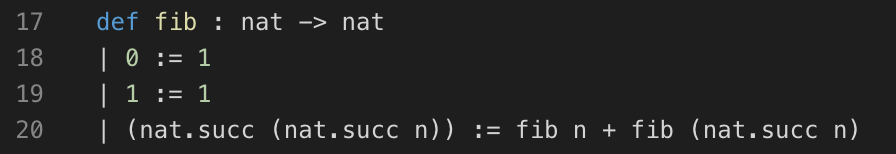
\includegraphics[width=\textwidth]{figures/fol_example_fib_definition.png}
		\caption{Sample inductive declaration}
		\label{fig:fol_example_declaration}
	\end{subfigure}
	\hspace{1mm}
	\begin{subfigure}{0.65\textwidth}
		\centering
		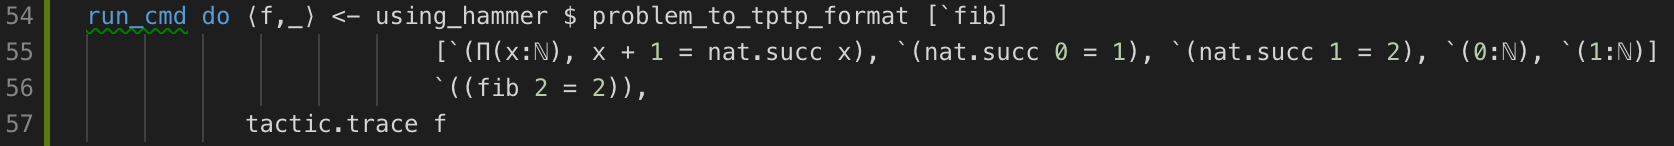
\includegraphics[width=\textwidth]{figures/fol_example_call.png}
		\caption{Sample translation problem}
		\label{fig:fol_example_translation}
	\end{subfigure}
	\caption{FOL translation example in Lean. The code can be found in the file \texttt{leanhammer.lean}. The left side shows the inductive declaration of \texttt{fib}, and the right the call for translating this into plain FOL in TPTP encoding. }
	\label{fig:fol_example}
\end{figure}

The main function that is used is \texttt{problem\_to\_tptp\_format}. This function takes as first argument a list of declarations that are eventually relevant for the conjecture and should be included in the translation. In our case, we want to translate the inductive declaration of the Fibonacci numbers as shown in Figure~\ref{fig:fol_example_declaration}. The second argument is a list of expressions that should be translated as clauses. Here, we for example have to define that 0 and 1 are natural numbers. If we would leave these out, we will not be able to find a proof as the clause implementing \texttt{fib} in FOL has as pre-condition that the argument is of type \texttt{nat}. The last expression we enter to the translation process is of course the conjecture. By tracing the output of the function, we see the translated construct in text form, which can be used for other theorem provers. \\

To use this translation, copy output to the file \texttt{test\_problem.tptp} (note that the name of the file can be changed).
Run a theorem prover like E \cite{EProver} on this file by executing the command \texttt{./eprover --auto --tptp3-in \textit{file/to/}test\_problem.tptp}. If everything worked out correctly, E finds a proof in a few milliseconds.
\subsection{Open issues}
\begin{itemize}
	\item Up till now, the user has to specify by himself which declarations and expressions should be translated besides the conjecture. This process should be automated by a retrieving all possible clauses/declarations that are somehow connected with the conjecture, and then filtering/ranking these to only take the $N$ most relevant ones. Code based on an old version of Lean can be found \href{https://github.com/robertylewis/relevance_filter/tree/dev_lean_reparam}{here}, and the file \texttt{premise\_selection.lean} might be a good starting point.
	\item The translation of inductive declarations works fine in the Lean hammer. However, plain declarations like:\\
	\texttt{def sum\_two (x:$\mathbb{N}$) (y:$\mathbb{N}$) :$\mathbb{N}$ := x+y}\\
	cause troubles in the translation problem. Lean represents these functions as lambda expressions although we need it in pi notation (for all \texttt{x} and \texttt{y}, \texttt{sum\_two x y = x + y}). This translation needs to be integrated into the hammer. For debugging, a quick fix is to write all declarations inductively.
	\item Currently, the interaction to the theorem prover is in a debug stage where the user needs to copy the output of Lean into a file, and run E on it. In future, this process should be automated by an IO import/export to theorem provers.
	\item In relation to the previous points, once the IO communication with the theorem provers is automated, a proof reconstruction needs to be implemented. This would help the user to understand the proof, and provide him a way of implementing this proof in Lean.
	\item Another missing point is the translation of inductive types like \texttt{list}. Currently, these types are not supported.
\end{itemize}


%%%%%%%%%%%%%%%%%%%%%
%%%%%%%%%%%%%%%%%%%%%
%%%%%%%%%%%%%%%%%%%%%

\newpage
\section{General pipeline}
\label{sec:general_pipeline}
To support theorem provers of different input levels (TF0, TF1, TH0, TH1), the generalized version of the Lean hammer is planed to follow a pipeline which successively translates the Dependent Type Theory to FOL. The pipeline is visualized in Figure~\ref{fig:pipeline}.
\begin{figure}[ht!]
	\centering
	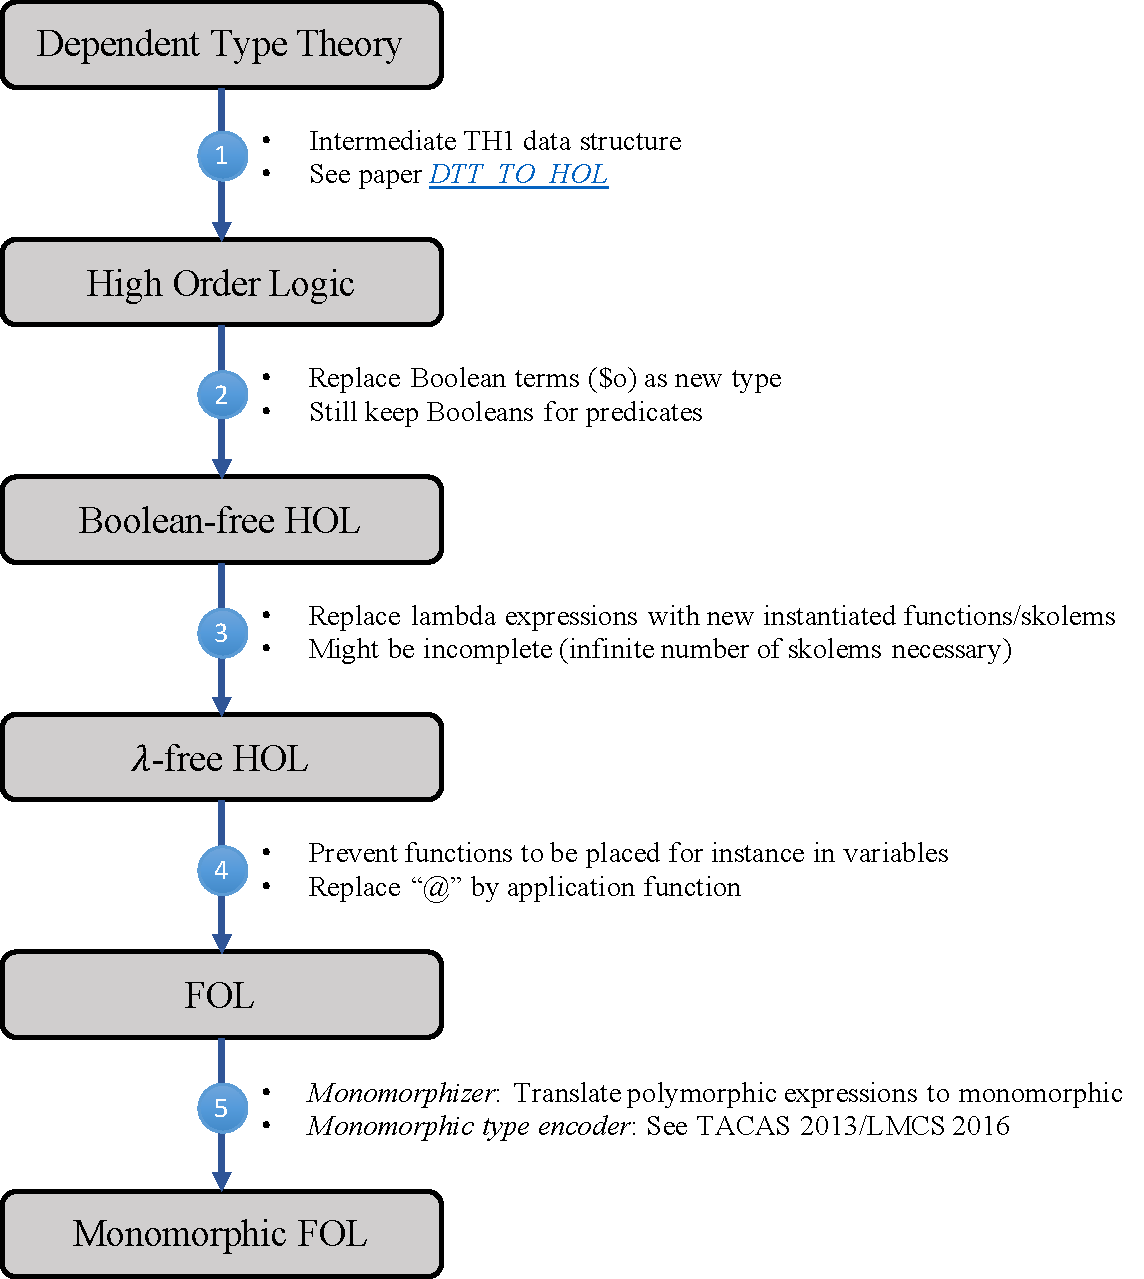
\includegraphics[width=0.45\textwidth]{figures/pipeline_DTT_HOL.pdf}
	\caption{General overview of the translation pipeline from Dependent Type Theory to different logic forms.}
	\label{fig:pipeline}
\end{figure}
\subsection{Dependent Type Theory to High Order Logic}
The first step of our pipeline is parsing the Dependent Type Theory of Lean to TH1. We decided to take TH1 as highest-level language as most high-order theorem prover can deal with this language. This section first describes the data structures itself, and then continues with discussing the translation process.

\subsubsection{Data structures} 
\begin{description}
	\item[holtype] The data structure \texttt{holtype} represents type expressions in TH1. The following types are distinguished:
	\begin{itemize}
		\item The standard types \texttt{\$o} (boolean), \texttt{\$i} (int) and \texttt{\$type} (type class) are implemented as constants
		\item Local types can be created by \texttt{ltype}. It is intended that these types are applied when using previously defined types in axioms. Example:
		\begin{verbatim}
			thf(bird_type, type, (bird : $tType)).
			thf(tweety_type, type, (tweety: bird)).
			...
		\end{verbatim}
		The usage of \texttt{bird} in the second type definition should be done by \texttt{ltype}. Note that the usage of \texttt{bird} in the first line is not included in a \texttt{holtype} data item, but in a full \texttt{type\_definition}. 
		\item \texttt{functor} provides support for defining functions with multiple parameters. Example:
		\begin{verbatim}
		thf(map_type, type, (map : $tType > $tType > $tType)).
		\end{verbatim}
		The functor type should be defined as:
		\begin{verbatim}
		holtype.functor [holtype.type, holtype.type] holtype.type
		\end{verbatim}
		Note that we use a list instead of a recursive structure in order to simplify encodings for other logic levels. In TF0 and TF1, we for example have to write: 
		\begin{verbatim}
		tff(map_type, type, (map : ($tType * $tType) > $tType)).
		\end{verbatim}
		\item The deep binder option is thought to be used for type signatures with type arguments. An example use-case is:
		\begin{verbatim}
		thf(bird_lookup_type, type, (bird_lookup: !>[A:$tType, B:$tType] : ((map@A@B) > A > B))).
		\end{verbatim}
		\item At last, we also need to support partial applications as term arguments. Thus, in the previous example, \texttt{map@A@B} should be encoded by \texttt{holtype.partial\_app}.
	\end{itemize}
	\item[holterm] Type
	\item[holform] Type
\end{description}
\subsubsection{Translation}
\textcolor{red}{In progress} (see this \href{https://link.springer.com/chapter/10.1007/BFb0037108}{paper} for translation of DTT to HOL \cite{DTT2HOL}). 
\subsection{High Order Logic to Boolean-free HOL}
\subsection{Boolean-free HOL to $\lambda$-free HOL}
\subsection{$\lambda$-free HOL to FOL}
\subsection{FOL to monomorphic FOL}

\newpage
\bibliographystyle{plain}
\bibliography{references.bib}

\appendix
\section{FOL examples}
\label{sec:fol_examples}
The non-optimized output for the example of proving that \texttt{fib 2 = 2} is shown below:

\footnotesize
\begin{verbatim}
fof('_fresh.265.4460',
axiom,
(t(a(a('has_one.one',
'nat'),
'nat.has_one'),
'nat'))).

fof('_fresh.265.4459',
axiom,
(t(a(a('has_zero.zero',
'nat'),
'nat.has_zero'),
'nat'))).

fof('_fresh.265.4455',
axiom,
((a(a(a('bit0',
'nat'),
'nat.has_add'),
a(a('has_one.one',
'nat'),
'nat.has_one'))
= a('nat.succ',
a(a('has_one.one',
'nat'),
'nat.has_one'))))).

fof('_fresh.265.4454',
axiom,
(t(a('nat.succ',
a(a('has_one.one',
'nat'),
'nat.has_one')),
'nat'))).

fof('_fresh.265.4453',
axiom,
((a(a('has_one.one',
'nat'),
'nat.has_one')
= a('nat.succ',
a(a('has_zero.zero',
'nat'),
'nat.has_zero'))))).

fof('_fresh.265.4452',
axiom,
(t(a('nat.succ',
a(a('has_zero.zero',
'nat'),
'nat.has_zero')),
'nat'))).

fof('_fresh.265.4450',
axiom,
(! [V1 /* _fresh.265.4451 */] :
((t(V1,
'nat'))
=> (t(a('fib',
V1),
'nat'))))).

fof('_fresh.265.4447',
axiom,
((a('fib',
a(a('has_zero.zero',
'nat'),
'nat.has_zero'))
= a(a('has_one.one',
'nat'),
'nat.has_one')))).

fof('_fresh.265.4444',
axiom,
((a('fib',
a(a('has_one.one',
'nat'),
'nat.has_one'))
= a(a('has_one.one',
'nat'),
'nat.has_one')))).

fof('_fresh.265.4437',
axiom,
(! [V1 /* _fresh.265.4438 */] :
((t(V1,
'nat'))
=> ((a('fib',
a('nat.succ',
a('nat.succ',
V1)))
= a(a(a(a('has_add.add',
'nat'),
'nat.has_add'),
a('fib',
V1)),
a('fib',
a('nat.succ',
V1)))))))).

fof('problem_conjecture',
conjecture,
((a('fib',
a(a(a('bit0',
'nat'),
'nat.has_add'),
a(a('has_one.one',
'nat'),
'nat.has_one')))
= a(a(a('bit0',
'nat'),
'nat.has_add'),
a(a('has_one.one',
'nat'),
'nat.has_one'))))).
\end{verbatim}

\normalsize
\subsection{Optimized FOL export}
\label{sec:fol_examples_optimized}
The optimized version get rids of some constant term applications, and replaces it with a new name. For debugging purpose, the names are right now the concatenation of the term names that were combined for the new constant:

\footnotesize
\begin{verbatim}
fof('_fresh.325.1061',
axiom,
(t('const_.a_.a_.c_.has_one.one.-.c_.nat.-.c_.nat.has_one',
'nat'))).

fof('_fresh.325.1060',
axiom,
(t('const_.a_.a_.c_.has_zero.zero.-.c_.nat.-.c_.nat.has_zero',
'nat'))).

fof('_fresh.325.1056',
axiom,
(('const_.a_.a_.a_.c_.bit0.-.c_.nat.-.c_.nat.has_add.-.c_.const_.a_.a_.c_.has_one.one.-.c_.nat.-.c_.nat.has_one'
= a('nat.succ',
'const_.a_.a_.c_.has_one.one.-.c_.nat.-.c_.nat.has_one')))).

fof('_fresh.325.1055',
axiom,
(t(a('nat.succ',
'const_.a_.a_.c_.has_one.one.-.c_.nat.-.c_.nat.has_one'),
'nat'))).

fof('_fresh.325.1054',
axiom,
(('const_.a_.a_.c_.has_one.one.-.c_.nat.-.c_.nat.has_one'
= a('nat.succ',
'const_.a_.a_.c_.has_zero.zero.-.c_.nat.-.c_.nat.has_zero')))).

fof('_fresh.325.1053',
axiom,
(t(a('nat.succ',
'const_.a_.a_.c_.has_zero.zero.-.c_.nat.-.c_.nat.has_zero'),
'nat'))).

fof('_fresh.325.1051',
axiom,
(! [V1 /* _fresh.325.1052 */] :
((t(V1,
'nat'))
=> ((a(a('const_.a_.a_.c_.has_add.add.-.c_.nat.-.c_.nat.has_add',
V1),
'const_.a_.a_.c_.has_one.one.-.c_.nat.-.c_.nat.has_one')
= a('nat.succ',
V1)))))).

fof('_fresh.325.1048',
axiom,
(! [V1 /* _fresh.325.1049 */] :
((t(V1,
'nat'))
=> (t(a('fib',
V1),
'nat'))))).

fof('_fresh.325.1045',
axiom,
((a('fib',
'const_.a_.a_.c_.has_zero.zero.-.c_.nat.-.c_.nat.has_zero')
= 'const_.a_.a_.c_.has_one.one.-.c_.nat.-.c_.nat.has_one'))).

fof('_fresh.325.1042',
axiom,
((a('fib',
'const_.a_.a_.c_.has_one.one.-.c_.nat.-.c_.nat.has_one')
= 'const_.a_.a_.c_.has_one.one.-.c_.nat.-.c_.nat.has_one'))).

fof('_fresh.325.1035',
axiom,
(! [V1 /* _fresh.325.1036 */] :
((t(V1,
'nat'))
=> ((a('fib',
a('nat.succ',
a('nat.succ',
V1)))
= a(a('const_.a_.a_.c_.has_add.add.-.c_.nat.-.c_.nat.has_add',
a('fib',
V1)),
a('fib',
a('nat.succ',
V1)))))))).

fof('problem_conjecture',
conjecture,
((a('fib',
'const_.a_.a_.a_.c_.bit0.-.c_.nat.-.c_.nat.has_add.-.c_.const_.a_.a_.c_.has_one.one.-.c_.nat.-.c_.nat.has_one')
= 'const_.a_.a_.a_.c_.bit0.-.c_.nat.-.c_.nat.has_add.-.c_.const_.a_.a_.c_.has_one.one.-.c_.nat.-.c_.nat.has_one'))).
\end{verbatim}
\end{document}